\section{Introduction}
\label{sec:intro}

Understanding the animals' verbal expressions is an interesting interdisciplinary scientific challenge, 
in particular pet dogs, who are closely integrated with humans. 
Previous research endeavors to comprehend dog barking sounds for a number of reasons, such as for a better understanding of animal biological evolution\cite{pongracz2017modeling}, applying their language to information technology, or just curiosity about dogs' intention when they bark~\cite{pongracz2011children,dogbark_1}. However, this task is challenging not only due to the unknown acoustic pattern of dogs, but also the lack of a high-quality dataset.

In this paper, we investigate dogs' verbal expressions, which is their barking sounds, one of the main communication channels. 
%define the language of dogs as their audio communication channel, which is barking. 
One ubiquitous feature of any communication channel is that it does evolve with the interaction 
between the environment and creatures around it\cite{arnold2018affect}. 
Previous research has demonstrated that dog's barking sound indeed reflects their intrinsic characteristics~\cite{pongracz2010barking,larranaga2015comparing}, emotional expression~\cite{thorndike2017animal,hantke2018my,paladini2020bark} and understanding of outsides~\cite{larranaga2015comparing, molnar2008classification}. 
%\KZ{What do you mean by reflecting scene understanding?}
However, little research has looked into the influence arising from the interaction between human hosts and dogs. 
In our work, we hypothesize that dogs' acoustic characteristics can be highly correlated with such interaction, particularly 
the host's language. 
%\KZ{Because our final conclusion is that dog voices are highly ``correlated'' with human linguistic features, we might not be able to say that dog language is ``shaped'' by the host language.}
To verify that, we explore the barking difference of a particular dog species (Shiba Inu) from 
two different host language environments (English vs. Japanese)~(\figref{fig:intropic}). Shiba Inu dogs are selected to be studied because there are a large number of related videos online for us to generate a dataset, at the same time, we choose English and Japanese host language environments as their phonetic systems have significant difference.%\MYW{Add 1-2 sentence to illustrate why we focus on these two languages, i.e. their phonetic system differ greatly}

\begin{figure}[t]
	\centering
	\scalebox{0.24}{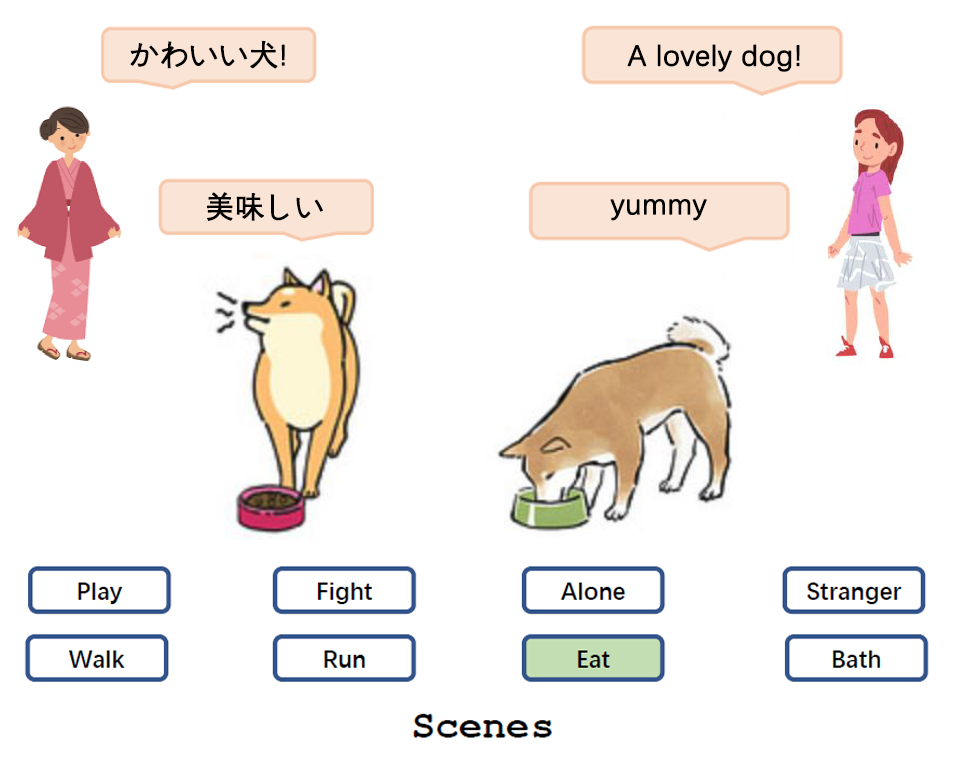
\includegraphics{intropic_big_add.png}}
	\caption{With the interaction between the hosts and the dogs, their acoustic sounds have a strong correlation.}%\KZ{Reconsider this caption: During the interaction between dogs and their hosts from different language environments, dog barking sounds are possible to be shaped.}
	\label{fig:intropic}
\end{figure}

Since there is no existing dataset, we first construct a dataset called ``EJShibaVoice.'' We choose to study Shiba Inu dogs because there are a large number of Shiba Inu dogs in Japanese and English-speaking communities. 
As YouTube features a large number of Shiba Inu dog videos, we designed a framework to crawl Shiba Inu audio clips from both English and Japanese-speaking host families with barking sound extraction and tag them with extra information including their language environments, activities, and recording locations. %\KZ{Do we have locations?} yes we have, we use a model to predict the locations. 
%\MYW{Activity scene & location are confusing, the recording location and dogs' activity instead?}

Then, we conducted classification experiments to check if there exists any interesting acoustic properties 
that distinguish dog barks from one language environment with the other. 
The classification experiment is performed on the clips paired with similar contexts to exclude some of the confounding non-linguistic factors. 
To explore the prominent acoustic features, 
multiple commonly-used audio features are utilized, including filterbank~\cite{strang1996wavelets}, 
ComParE~\cite{schuller2013interspeech}, GeMAPS, eGeMAPS~\cite{eyben2015geneva}, 
PLP~\cite{eyben2015geneva} and MFCC~\cite{davis1980comparison}.


% mfcc~\cite{davis1980comparison}, mel spectrogram, GeMAPS~\cite{eyben2015geneva}, filterbank~\cite{strang1996wavelets} and PLP~\cite{hermansky1990perceptual}. 

% In the meantime, as barks of dogs are influenced by the scenes, we try to reduce such kind of noise by doing experiment on specific scenes. Some interesting differences were discovered.\MYW{What is this sentence about? Either say more about the differences or cut it out.}

Finally, to discover the most prominent factors that distinguish dog barks by their language environment, 
we perform an importance analysis of different factors using Shapley values. The fact that several most important factors have substantial correlations with the acoustic characteristics of the hosts' language (i.e., English or Japanese) supports our hypothesis that the host language environment does have a strong correlation with dogs' barking sounds.

Our contributions are summarized as follows:

\begin{itemize}
	\item We define a new task to discover the human linguistic influence on the vocal expression
	(barks) of Shiba Inu dogs, which can inspire further research on animal languages.~(\secref{sec:assumption})
	\item We construct a Shiba Inu barks dataset \textbf{EJShibaVoice} with 7,907 audio clips, 
	produced by dogs from two different language environments: English and Japanese. The dataset also contains the corresponding 54,142 host speech clips.~(\secref{sec:assumption})
	\item We discovered prominent acoustic differences between dogs from different language environments: 
	Shiba Inus under English host language environments have a lower frequency, while those under Japanese environments have shorter duration, which correlates with 
	corresponding host languages.~(\secref{sec:main})%by testing several kinds of audio features on our pairwise dataset.
\end{itemize}